\chapter[Análise dos Resultados]{Análise dos Resultados}\label{ch:analiseResultados}
  Este capítulo tem como objetivo discutir  os resultados obtidos durante a realização dos testes. Dentre estes
resultados, estão presentes as fontes de erros levantadas com a experiência do desenvolvimento,
suas respectivas correções, dentro do possível, e a análise da viabilidade da utilização do
sistema no contexto da reabilitação motora. Desse modo, este
capítulo está dividido nas seções: Testes(\ref{sol:solucao}) e Fontes de erro(\ref{sol:fontesErro}).

\section{Testes}\label{sec:testes}
  O principal objetivo dos testes é a observação e a análise do sistema. Após a realização de todos os testes propostos, foi possível chegar a
uma conclusão quanto à viabilidade da utilização do sistema no contexto da reabilitação motora,
 a qual será apresentada na seção \ref{sol:viabilidade}.

 Os testes consistem em cinco situações, nas quais a solução foi analisada,
variando entre elas o movimento e ambiente. Buscando analisar os resultados obtidos em cada contexto.

  Os dados obtidos em cada teste está estruturado de acordo com a tabela \ref{tab:analise}.

  \begin{table}[H]
  \centering
  \caption{Estruturação dos Dados}
  \label{tab:analise}
  \begin{tabular}{@{}|l|l|l|l|l|@{}}
  \toprule
  \textbf{Ex} &\textbf{Movimento} & \textbf{Complexidade} & \textbf{Luz ambiente} & \textbf{exatidão} \\ \bottomrule
  \end{tabular}
  \end{table}

\begin{itemize}
  \item \textbf{Ex}: Número de execução do teste. Cada teste foi executado três vezes.
  \item \textbf{Movimento}: O nome e descrição do movimento análisado, \textbf{exemplo}: Levantar e abaixar braço direito.
  \item \textbf{Complexidade}: Essa variável é referente a complexidade da execução do movimento, para o mapeamento do \textit{kinect} e acompanhamento do usuário.
   A rotulação dessa variável segue a tabela \ref{tab:compl}.

    \begin{table}[H]
    \centering
    \caption{Rotulação da complexidade do Movimento}
    \label{tab:compl}
    \begin{tabular}{@{}|c|c|@{}}
\toprule
\textbf{Complexidade} & \textbf{Descrição}                                                                                                                                          \\ \midrule
\textbf{Alta}         & \begin{tabular}[c]{@{}c@{}}Execução do movimento é de difícil mapeamento para \\ o kinect e para acompanhamento do usuário.\end{tabular}                    \\ \midrule
\textbf{Media}        & \begin{tabular}[c]{@{}c@{}}Execução do movimento é de dificuldade moderada para\\ o mapeamento para o kinect e para acompanhamento do usuário.\end{tabular} \\ \midrule
\textbf{Baixa}        & \begin{tabular}[c]{@{}c@{}}Execução do movimento é de dificuldade baixa para\\  o mapeamento para o kinect e para acompanhamento do usuário.\end{tabular}   \\ \bottomrule
\end{tabular}
\end{table}

  \item \textbf{Luz ambiente}: Com a premissa básica de um ambiente com pelo menos um metro e meio do sensor, essa variável diz respeito
a intensidade da luminosidade do ambiente, podendo ser \textbf{boa}, \textbf{regular} e \textbf{ruim}.

  \item \textbf{Exatidão}: Essa variável é referente a exatidão que o \textit{kinect} acompanha e corrige o movimento do usuário.
   A rotulação dessa variável segue a tabela \ref{tab:compl}.
    \begin{table}[H]
    \centering
    \caption{Rotulação da complexidade do Movimento}
    \label{tab:compl}
    \begin{tabular}{@{}|c|c|@{}}
\toprule
\textbf{Exatidão} & \textbf{Descrição}                                                                                                        \\ \midrule
\textbf{Boa}      & \begin{tabular}[c]{@{}c@{}}Bom acompanhamento e correção no movimento\\  executado pelo usuário\end{tabular}              \\ \midrule
\textbf{Regular}  & \begin{tabular}[c]{@{}c@{}}Regular acompanhamento e correção no movimento\\  executado pelo usuário.\end{tabular}         \\ \midrule
\textbf{Ruim}     & \begin{tabular}[c]{@{}c@{}}Ruim ou péssimo acompanhamento e correção no movimento\\  executado pelo usuário.\end{tabular} \\ \bottomrule
\end{tabular}
\end{table}

\end{itemize}


  As seções \ref{sub:teste1},\ref{sub:teste2} e \ref{sub:teste3}, apresentam os testes com diferentes variáveis, possibilitando a ánalise do comportamento do sistema em tais
  casos. Todos os testes foram feitos em um ambiente com quatro metros quadrados e o sensor \textit{kinect} em uma altura de aproximadamente um metro e meio.

\subsection{Teste 1}\label{sub:teste1}
  Os resultados obtidos com o teste estão dispostos na tabela \ref{tab:teste1}. Esse teste consiste no levantamento do braço direito, em uma velocidade
  baixa.


\begin{table}[H]
\centering
\caption{Teste 1}
\label{tab:teste1}
\begin{tabular}{@{}|c|c|l|l|l|@{}}
\toprule
\multicolumn{1}{|l|}{\textbf{Ex}} & \multicolumn{1}{l|}{\textbf{Movimento}} & \textbf{Complexidade} & \textbf{Luz Ambiente} & \textbf{Exatidão} \\ \midrule
1                                 & Levantar Braço Dir.                     & Baixa                 & Boa                   & Boa               \\ \midrule
2                                 & Levantar Braço Dir.                     & Baixa                 & Regular               & Regular           \\ \midrule
3                                 & Levantar Braço Dir.                     & Baixa                 & Ruim                  & Ruim              \\ \bottomrule
\end{tabular}
\end{table}

  Como pode ser observado na tabela \ref{tab:teste1} que a luz ambiente tem grande influência no mapeamento do \textit{kinect}, isso era esperado
já que a forma que ele faz a captação do ambiente é baseado em suas câmeras. Podemos observar na imagem \ref{img:teste1}, o esqueleto à esquerda é o movimento
que está sendo executado pelo usuário, assim o movimento tem que ser executado
com certa fidelidade, caso contrário os erros serão apresentados na forma de esferas sobre as juntas que se devem ser corrigidas. E na imagem \ref{img2:teste1} a correta execução do movimento.

\begin{figure}[H]
\centering
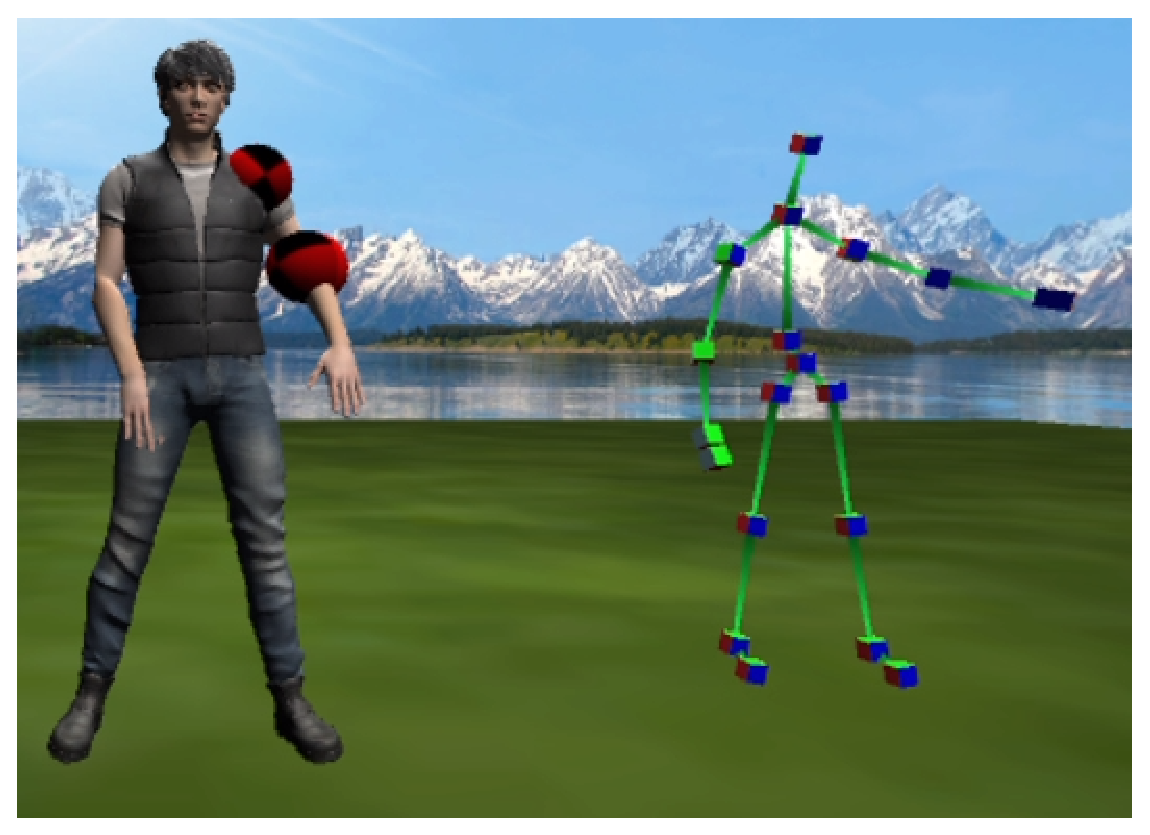
\includegraphics [keepaspectratio=true,scale=0.60]{figuras/img2teste1.eps}
\caption{Movimento com presença de falhas}
\label{img:teste1}
\end{figure}

\begin{figure}[H]
\centering
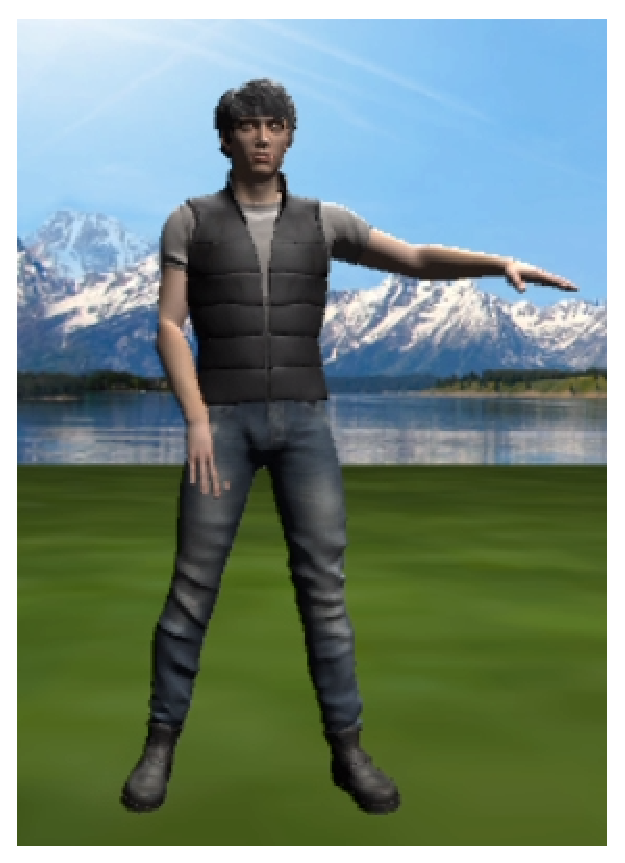
\includegraphics [keepaspectratio=true,scale=0.60]{figuras/imgteste1.eps}
\caption{Movimento correto}
\label{img2:teste1}
\end{figure}


\subsection{Teste 2}\label{sub:teste2}
Os resultados obtidos com o teste estão dispostos na tabela \ref{tab:teste2}. Esse teste consiste no levantamento dos dois braços , em uma velocidade
baixa.


\begin{table}[H]
\centering
\caption{Teste 2}
\label{tab:teste2}
\begin{tabular}{@{}|c|c|l|l|l|@{}}
\toprule
\multicolumn{1}{|l|}{\textbf{Ex}} & \multicolumn{1}{l|}{\textbf{Movimento}} & \textbf{Complexidade} & \textbf{Luz Ambiente} & \textbf{Exatidão} \\ \midrule
1                                 & Levantar os  Braços                     & Baixa                 & Boa                   & Boa               \\ \midrule
2                                 & Levantar os  Braços                     & Baixa                 & Regular               & Regular           \\ \midrule
3                                 & Levantar os  Braços                     & Baixa                 & Ruim                  & Ruim              \\ \bottomrule
\end{tabular}
\end{table}Corroboramos

Como pode ser observado na tabela \ref{tab:teste2} a luz ambiente tem grande influência no mapeamento do \textit{kinect}, porém com uma luz ambiente boa
a exatidão do sensor é \textbf{boa}.

\subsection{Teste 3}\label{sub:teste3}
Os resultados obtidos com o teste estão dispostos na tabela \ref{tab:teste3}. Esse teste consiste em sentar e levantar em uma cadeira , em uma velocidade
baixa.


\begin{table}[H]
\centering
\caption{Teste 3}
\label{tab:teste3}
\begin{tabular}{@{}|c|c|l|l|l|@{}}
\toprule
\multicolumn{1}{|l|}{\textbf{Ex}} & \multicolumn{1}{l|}{\textbf{Movimento}} & \textbf{Complexidade} & \textbf{Luz Ambiente} & \textbf{Exatidão} \\ \midrule
1                                 & Levantar os  Braços                     & Alta                 & Boa                   & Ruim               \\ \midrule
2                                 & Levantar os  Braços                     & Alta                 & Regular               & Ruim           \\ \midrule
3                                 & Levantar os  Braços                     & Alta                 & Ruim                  & Ruim              \\ \bottomrule
\end{tabular}
\end{table}

Como pode ser observado na tabela \ref{tab:teste3} o \textit{kinect} não consegue mapear bem uma pessoa de lado, o sensor se perde nas referências mostrando isntabilidade como pode ser
visto na imagem \ref{img:teste3}.

\begin{figure}[H]
\centering
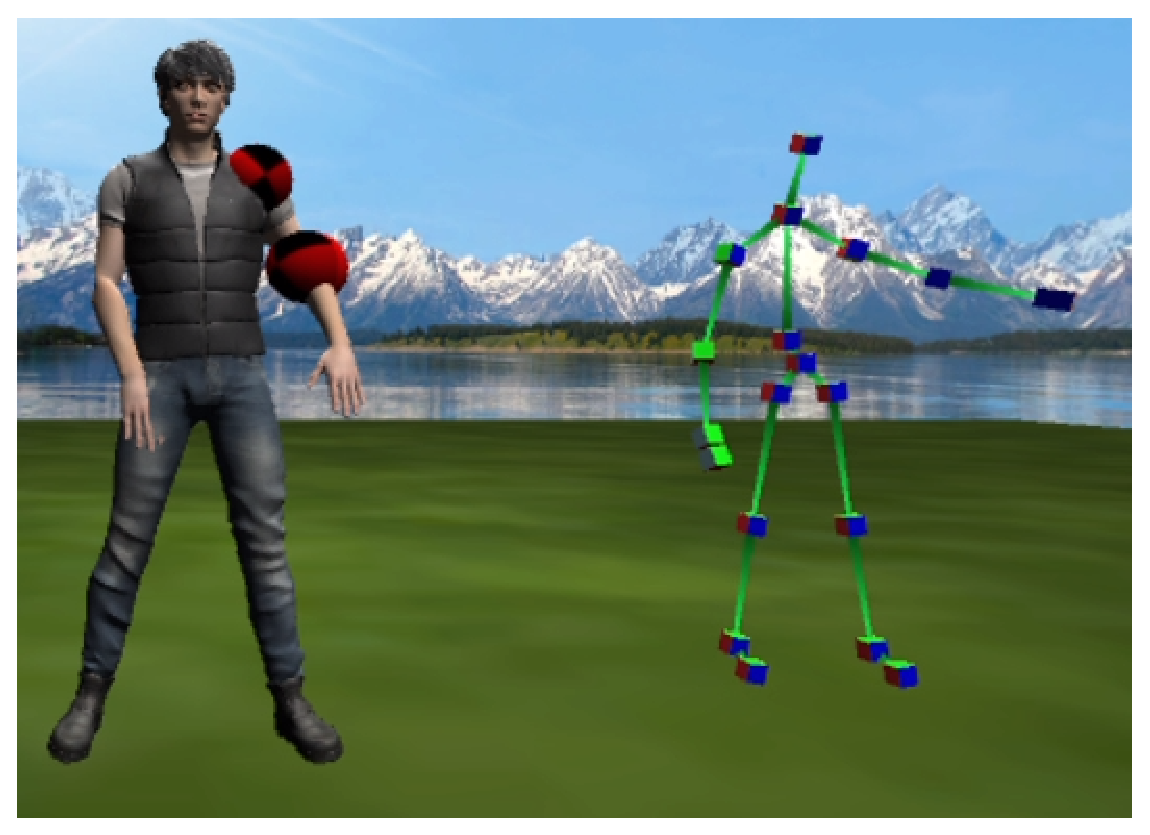
\includegraphics [keepaspectratio=true,scale=0.60]{figuras/img2teste1.eps}
\caption{Dados das articulações}
\label{img:teste3}
\end{figure}

\section{Fontes de Erro}\label{sol:fontesErro}
  Como já mencionando anteriormente, a principal fonte do erro do sistema é devido as limitações do \textit{kinect}, seja pela precisão ou pela luz do ambiente
. Por este motivo, é aconselhavel durante a execução dos movimentos o ambiente seja bem iluminado. Quanto a precisão,
durante a realização do desenvolvimento buscou-se minimizar a margem de erro do sensor, deixando uma maior área de graus sobre o movimento das juntas que não comprometesse de fato o movimento.

\section{Viabilidade}\label{sol:viabilidade}
  Com os testes vemos que sistema gerado com este trabalho é um produto acessível para a reabilitação motora, porém em casos onde não é ncessáro
fazer movimentos muito complexos e nem que exiga auxílio de objetos. Sendo melhor aplicado a reabilitação onde envolvam crianças, já que torna o processo
menos tedioso e mais lúdico.
